%
% hermite.tex -- 
%
% (c) 2021 Prof Dr Andreas Müller, OST Ostschweizer Fachhochschule
%
\bgroup
\begin{frame}[t]
\setlength{\abovedisplayskip}{5pt}
\setlength{\belowdisplayskip}{5pt}
\frametitle{Hermite-Polynome}
\vspace{-20pt}
\begin{columns}[t,onlytextwidth]
\begin{column}{0.68\textwidth}
\begin{center}
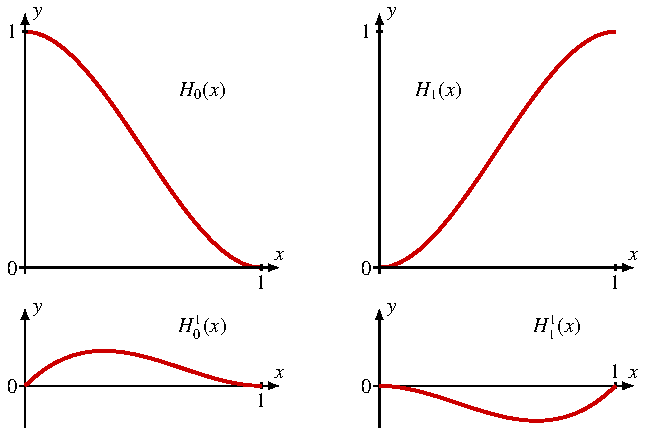
\includegraphics[width=\textwidth]{../../buch/chapters/030-nichtdiff/images/hermite.pdf}
\end{center}
\end{column}
\begin{column}{0.28\textwidth}
\begin{center}
\begin{tabular}{|>{$}l<{$}|>{$}c<{$}>{$}c<{$}|}
\hline 
f(x)  &f(0) & f(1)\llap{\raisebox{3pt}{\strut}} \\[3pt]
\hline
H_0(x)&   1 &    0\llap{\raisebox{3pt}{\strut}} \\
H_1(x)&   0 &    1 \\
H_0(x)&   0 &    0 \\
H_1(x)&   0 &    0 \\[3pt]
\hline
H_0^{1\prime}(x)&   0 &    0\llap{\raisebox{3pt}{\strut}} \\
H_1^{1\prime}(x)&   0 &    0 \\
H_0^{1\prime}(x)&   1 &    0 \\
H_1^{1\prime}(x)&   0 &    1 \\[3pt]
\hline
\end{tabular}
\end{center}
\end{column}
\end{columns}
\end{frame}
\egroup
